%---------------------------------------------------------------------
% Course 	: Introdunction To websciences
% Professor : Dr.Nelson
% Name   	: Babitha Bokka
% Assignment: 2
%---------------------------------------------------------------------
\documentclass[12pt]{article}
%--------------------------------------------------------------------
% packages required
%--------------------------------------------------------------------
\usepackage{graphicx}
\usepackage{listings}
\usepackage{hyperref}
\usepackage{caption}
\usepackage{color}
\graphicspath{ {images/} }
%--------------------------------------------------------------------
% Start Margins
%--------------------------------------------------------------------
\addtolength{\oddsidemargin}{-.875in}
\addtolength{\evensidemargin}{-.875in}
\addtolength{\textwidth}{1.75in}
\addtolength{\topmargin}{-.885in}
\addtolength{\textheight}{1.95in}
%-------------------------------------------------------------------
% End Margins
%--------------------------------------------------------------------
\definecolor{codegreen}{rgb}{0,0.6,0}
\definecolor{codegray}{rgb}{0.5,0.5,0.5}
\definecolor{codepurple}{rgb}{0.58,0,0.82}
\definecolor{backcolour}{rgb}{0.95,0.95,0.92}
 
\lstdefinestyle{mystyle}{
    backgroundcolor=\color{backcolour},   
    commentstyle=\color{codegreen},
    keywordstyle=\color{magenta},
    numberstyle=\tiny\color{codegray},
    stringstyle=\color{codepurple},
    basicstyle=\footnotesize,
    breakatwhitespace=false,         
    breaklines=true,                 
    captionpos=b,                    
    keepspaces=true,                 
    numbers=left,                    
    numbersep=5pt,                  
    showspaces=false,                
    showstringspaces=false,
    showtabs=false,                  
    tabsize=2
}
 
\lstset{style=mystyle}

\begin{document}

%---------------------------------------------------------------------
%Making the title page
%---------------------------------------------------------------------
\begin{titlepage}
\title{INTRODUCTION TO WEB SCIENCES:\\*Assignment 2}
\author{Babitha Bokka}
\date{28 September 2014}
\maketitle
\end{titlepage}

%---------------------------------------------------------------------
%Table of contents
%---------------------------------------------------------------------
\tableofcontents
\newpage
%------------------------------------------------------------------
%Question 1
%------------------------------------------------------------------
\section{Question 1}


To extract 1000 unique URIs from twitter based on a searching Keyword and URIs should be non-redirecting.
\subsection{Approach Towards the Solution}
I started solving this problem with the search keyword `noodles'. I requested the four keys required to interact with the twitter API and searched for the keyword by using the TwitterSearchOrder() function. I extracted the expanded URIs from the JSON. I saved all the URIs into a file, and then filtered them by using the Python set datatype, which eliminates all duplicates. I grabbed only the URIs which returned the HTTP 200 Response (ok) to eliminate any redirection.
\\*\\*
Note: In order to run the program, erase the existing finalUniqueUri.txt. All results are appended to the file which gives combines results from multiple runs.

\subsubsection{Desciption of searchTwitter.py}
\begin{enumerate}
	\item Use TwitterSearchOrder()to search the Twitter API.
	\item Choose a keyword to search.
	\item Look for keyword in all tweets.
	\item If there is a match then extract the expanded URL.
	\item Save the extracted URL to extractedUri.txt.
	\item extractedUri.txt has all non unique URLs.
\end{enumerate}
\subsubsection{Desciption of filterTwitter.py}
\begin{enumerate}
	\item Open the file and read each URL.
	\item Request the URL.
	\item Get the HTTP Response.
	\item If the status code is 200(OK), save the URL to finalUniqueUri.txt.
	\item finalUniqueUri.txt contains 1000 unique URLs.
\end{enumerate}

\newpage
\subsection{Source Code}
\subsubsection{searchTwitter.py}
\lstinputlisting[breaklines=True,language=Python]{../Q1/searchTwitter.py}
\subsubsection{filterTwitter.py}
\lstinputlisting[breaklines=True,language=Python]{../Q1/filterTwitter.py}
\newpage
\subsection{OutputFiles}
A sample of unique URI's :
\subsubsection{finalUniqueUri.txt}
\lstinputlisting[breaklines=True]{../Q1/urlFinalForDoc.txt}

%------------------------------------------------------------------
%Question 2
%------------------------------------------------------------------
\newpage
\section{Question 2}

To extract the timemaps of the 1000 unique URLs extracted obtained in Question 1 and count the number of mementos for each URL. Each memento represents a date and time where an individual URL was modified.

\subsection{Approach Towards the Solution}
To find the number of mementos, I used regular expressions (regexp) to locate the strings rel="memento" and rel="timemap". Occurances of the string rel="memento" were recorded to obtain a count of mementos for each URL. If there was a line containing rel="timemap", another page of mementos was available. I looped through each momento page until all mementos were counted. I then stored the results (mometo count, URL) in a text file.
\subsubsection{momentoTwitter.py}
\begin{enumerate}
	\item Open finalUniqueUri.txt .
	\item Read each URL.
	\item Append it to http://mementoweb.org/timemap/link/ .
	\item Request the complete URL.
	\item Get the response, and count the number of mementos.
	\item Check if there is a timemap line.
	\item If a timemap line is encountered, loop and collect all  momentos.
	\item Store the results to momentoUri.txt .
\end{enumerate}
\newpage
\subsection{Source Code}
\subsubsection{momentoTwitter.py}
\lstinputlisting[breaklines=True,language=Python]{../Q2/momentoTwitter.py}
\newpage
\subsection{OutputFiles}
\subsubsection{momentoUri.txt}
\lstinputlisting[breaklines=True]{../Q2/momentoForDoc.txt}
\newpage
%------------------------------------------------------------------
% Histogram
%------------------------------------------------------------------
\subsection{Histogram }
\subsubsection{code to generate the Histogram histogramCode.txt}
\lstinputlisting[breaklines=True]{../Q2/histogramCode.txt}
\subsubsection{Description of Histograms}
Figure \ref{fig:initial-histogram} represents mementos vs URI. If you observe the initial histogram, it does not give you a clear picture how many URIs have how many momentos.

The scaled histogram, Figure \ref{fig:scaled-histogram}, provdes additional insight about URIs and respective mementos.

\begin{figure}[ht]
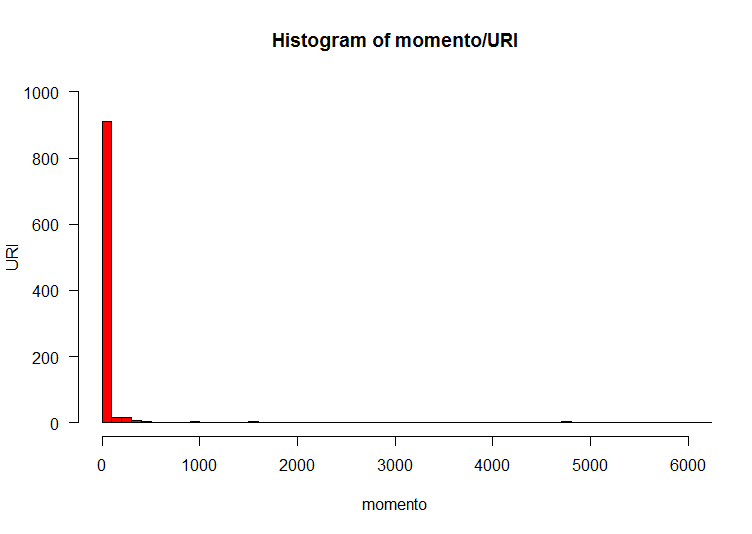
\includegraphics[scale=0.7]{../Q2/histogramMomentoURI_1}
\centering
\caption{Intial-histogram}
\label{fig:initial-histogram}
\end{figure}
\newpage
\begin{figure}[ht]
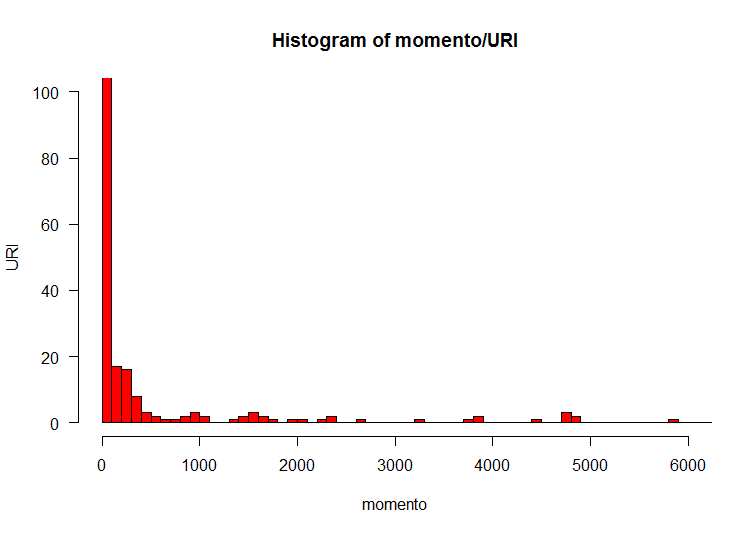
\includegraphics[scale=0.7]{../Q2/histogramMomentoURI_2}
\centering
\caption{Scaled-histogram}
\label{fig:scaled-histogram}
\end{figure}
\newpage
%------------------------------------------------------------------
%Question 3
%------------------------------------------------------------------
\section{Question 3}

Estimate the age of the each unique url by using the carbon date tool.
\subsection{Approach Towards the Solution}

To estimate the carbon date(estimated creation date) of each URL we download the carbondate tool files and run local.py get the creation dates and store them to a carbondateDays.txt.

CarbonDateTwitter.txt has the carbon date and URL, to estimate the age of the each url till today (date it was created and to till date gives us the number of days the url has been created) program daysCountTwitter.py will read each line and parses the date and estimates the number of days.

Relation between the memento and days can be obtained by running momentoDays.py which uses dictionary to store all the days and URL from carbonDateDays.txt for each URL it reads momentoUri.txt and checks whether there is a URL with greater than 0 momentos if it encounters any of the URL then that memento is appended to the dictionary.Then the results(days--momento) are stored in momentoDays.txt .
\subsubsection{description of daysCountTwitter.py}
\begin{enumerate}
	\item Modify the local.py extract the dates for each URL.
	\item Store in carbonDateTwitter.txt.
	\item Now load the file in to daysCountTwitter.py.
	\item Program calculates the number of days it has been since the URL has been created .
	\item Store the days and URL into carbonDateDays.txt.	
\end{enumerate}
\subsubsection{description of momentoDays.py}
\begin{enumerate}
	\item Open the file momentoDays.txt.
	\item Store the days and URL into a dictionary with key as URL {key:URL value :list[date]} value as days.	
	\item Now open the momentoUri.txt .
	\item Read each line and compare the URL with the dictionary key URL if there is a match and the number of mementos for that URL is greater that zero store the URL in momentoDays.txt.
	\item momentoDays.txt has days , mementos.
\end{enumerate}

\newpage
\subsubsection{daysCountTwitter.py}
\lstinputlisting[breaklines=True,language=Python]{../Q3/daysCountTwitter.py}
\newpage
\subsubsection{momentoDays.py}
\lstinputlisting[breaklines=True,language=Python]{../Q3/momentoDays.py}
\newpage
\subsection{OutputFiles}
\subsubsection{carbonDateTwitter.txt}
\lstinputlisting[breaklines=True]{../Q3/carbonForDoc.txt}
\subsubsection{carbonDateDays.txt}
\lstinputlisting[breaklines=True]{../Q3/carbonDaysForDoc.txt}
\subsubsection{momentoDays.txt}
\lstinputlisting[breaklines=True]{../Q3/momentoDaysForDoc.txt}
\newpage


\subsection{Scatterplot}
\subsubsection{Code to generate the Scatterplot scatterplotCode.txt}
\lstinputlisting[breaklines=True]{../Q3/scatterplotCode.txt}
\subsubsection{Description of Histogram}
Figure \ref{fig:initial-histogram} brings up the relation between the days and the memento.Figure \ref{fig:initial-histogram} and Figure \ref{fig:scaled-histogram} are plotted on the same data but Figure \ref{fig:scaled-histogram} gives additional insight. 

\begin{figure}[ht]
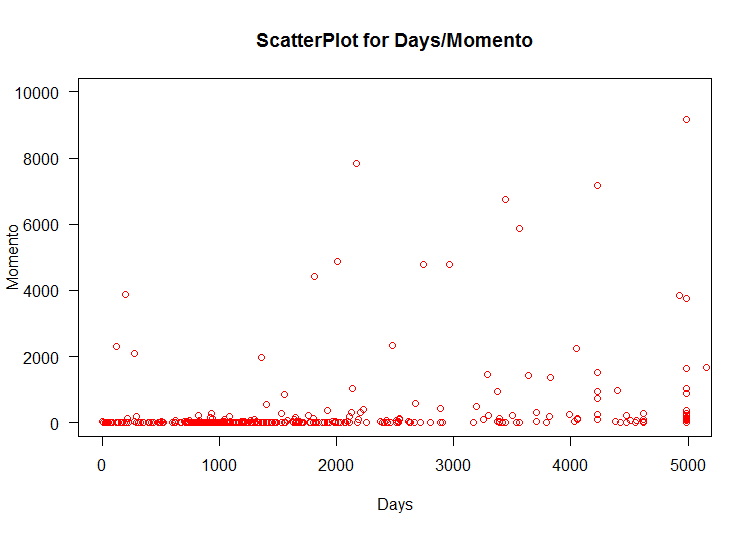
\includegraphics[scale=0.7]{../Q3/scatterDaysMomento_1}
\centering
\caption{intial scatterplot}
\label{intial-scatterplot}
\end{figure}
\newpage

\begin{figure}[ht]
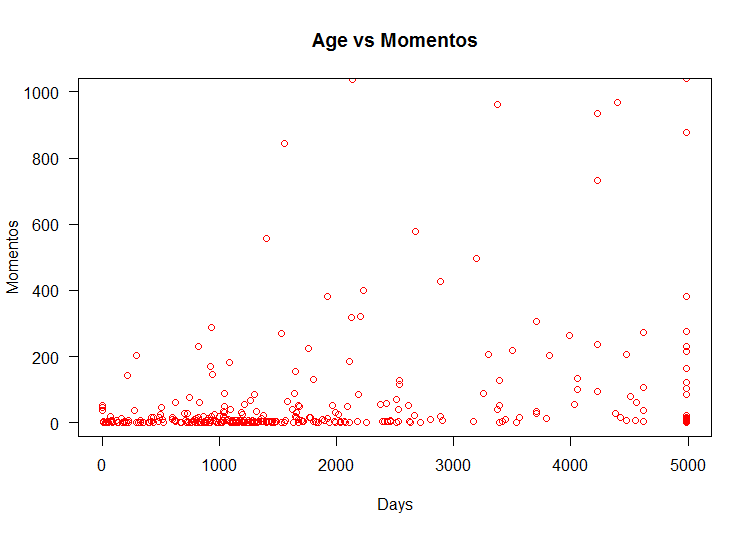
\includegraphics[scale=0.7]{../Q3/scatterDaysMomento_2}
\centering
\caption{Scaled scatterplot}
\label{scaled-scatterplot}
\end{figure}
\newpage
%-------------------------------------------------------------------
%References
%-------------------------------------------------------------------
\bibliographystyle{plain}
\bibliography{A2_report}
\cite{*}
\end{document}